\section{Contact Angle Measurement}

A contact angle can be defined for a triple-phase interface, where a solid, a liquid and a gas or vapor phase meet at a single point and are at an equilibrium. This is the case for a liquid drop resting on a surface (static equilibrium) or a liquid in a pipe (dynamic equilibrium). The contact angle is the angle at the triple phase interface between the solid-gas interface and the tangent of the liquid-gas or liquid-vapor interface.

\subsection{Underlying Theory}

The contact angle is a useful measure of the wetting characteristics of a material. A low contact angle characterizes a hydrophilic surface, whereas a high contact angle characterizes a hydrophobic surface. 
A drop resting on a smooth solid surface is an example of a static equilibrium triple-phase interface. The interfacial energies must therefore be in equilibrium, with gravity, and with each other. Let $\gamma_{LG}$, $\gamma_{SG}$ and $\gamma_{SL}$ be the respective liquid-gas, solid-gas and solid-liquid interfacial energies. We now consider an ideal solid-liquid-gas triple-phase boundary as depicted in figure \ref{fig:triple phase}, with $\theta$ the contact angle. Without loss of generality we consider a 2 dimensional system. To obtain the equilibrium contact angle we consider a small perturbation of the displayed system. We expand the liquid solid interface by a small distance $\Delta x$ and consider the changes in energy.

\begin{equation}
\Delta E = \gamma_{SL}\, \Delta x + \gamma_{SG} \, ( - \Delta x) + \gamma_{LG} \cos{\theta} \, \Delta x
\end{equation}

at equilibrium we expect this change to be congruent to zero, hence we obtain the following energy balance.

\begin{equation}
\gamma{SG} \, \Delta x = \gamma_{SL} \, \Delta x + \gamma_{LG} \cos{\theta}\, \Delta x
\end{equation}

By eliminating the common factor $\Delta x$ we obtain a surface energy balance equation for the triple-phase boundary known as Young's equation:


\begin{equation}
\gamma{SG} = \gamma_{SL} + \gamma_{LG} \cos{\theta}
\end{equation}

Deviations from the ideal behavior associated with Young's equation can be attributed to the roughness of a non ideal surface. These can be accounted for by applying either the Wenzel or Cassie equations for homogeneous and heterogeneous surfaces respectively. In the context of this experiment we contend ourselves with the simpler model reflected in Young's equation (our samples are relatively planar).
For dynamic situations (for example water running down a windowpane) the situation is further complicated. In this case one must differentiate between the advancing and receding contact angles. As with the previous complications we will focus on a system where such effect need not be considered i.e. a stationary drop.

\subsection{Measurement Procedure}

The contact angle measurements where performed optically by observing a droplet of deionized water on different samples prepared in the manner described in section II. For this purpose the the sample was placed on a three degree of freedom (linear) movable stage. The water droplets were provided by a servo driven syringe of deionized water. We setup the syringe to dispense 3 $\mu \ell$ of water. Subsequently we raised the sample until the drop made contact with, and participated onto the sample. 

We measured the contact angle at least 5 times on each sample using the above mentioned contact angle measurement device. After dropping a liquid on the surface of the sample, we plotted the liquid drop profiles and extrapolated the contact angles. Subsequently we Analyzed experiment data by calculating the mean values and the errors. The results will be presented in the next section.

\subsection{Results and Analysis}

The results from the contact angle measurement are shown in figure \ref{fig:results}. Sample 1 is clearly more hydrophilic than Sample 2, as evidenced by the difference contact angle well beyond the error. As expected the mixed sample exhibited intermediate wetting characteristics. However the large error in the measurement does not permit any conclusions on which thiol contributes more to the wetting characteristics.

\begin{figure}
\centering
% GNUPLOT: LaTeX picture with Postscript
\begingroup
  \makeatletter
  \providecommand\color[2][]{%
    \GenericError{(gnuplot) \space\space\space\@spaces}{%
      Package color not loaded in conjunction with
      terminal option `colourtext'%
    }{See the gnuplot documentation for explanation.%
    }{Either use 'blacktext' in gnuplot or load the package
      color.sty in LaTeX.}%
    \renewcommand\color[2][]{}%
  }%
  \providecommand\includegraphics[2][]{%
    \GenericError{(gnuplot) \space\space\space\@spaces}{%
      Package graphicx or graphics not loaded%
    }{See the gnuplot documentation for explanation.%
    }{The gnuplot epslatex terminal needs graphicx.sty or graphics.sty.}%
    \renewcommand\includegraphics[2][]{}%
  }%
  \providecommand\rotatebox[2]{#2}%
  \@ifundefined{ifGPcolor}{%
    \newif\ifGPcolor
    \GPcolortrue
  }{}%
  \@ifundefined{ifGPblacktext}{%
    \newif\ifGPblacktext
    \GPblacktexttrue
  }{}%
  % define a \g@addto@macro without @ in the name:
  \let\gplgaddtomacro\g@addto@macro
  % define empty templates for all commands taking text:
  \gdef\gplbacktext{}%
  \gdef\gplfronttext{}%
  \makeatother
  \ifGPblacktext
    % no textcolor at all
    \def\colorrgb#1{}%
    \def\colorgray#1{}%
  \else
    % gray or color?
    \ifGPcolor
      \def\colorrgb#1{\color[rgb]{#1}}%
      \def\colorgray#1{\color[gray]{#1}}%
      \expandafter\def\csname LTw\endcsname{\color{white}}%
      \expandafter\def\csname LTb\endcsname{\color{black}}%
      \expandafter\def\csname LTa\endcsname{\color{black}}%
      \expandafter\def\csname LT0\endcsname{\color[rgb]{1,0,0}}%
      \expandafter\def\csname LT1\endcsname{\color[rgb]{0,1,0}}%
      \expandafter\def\csname LT2\endcsname{\color[rgb]{0,0,1}}%
      \expandafter\def\csname LT3\endcsname{\color[rgb]{1,0,1}}%
      \expandafter\def\csname LT4\endcsname{\color[rgb]{0,1,1}}%
      \expandafter\def\csname LT5\endcsname{\color[rgb]{1,1,0}}%
      \expandafter\def\csname LT6\endcsname{\color[rgb]{0,0,0}}%
      \expandafter\def\csname LT7\endcsname{\color[rgb]{1,0.3,0}}%
      \expandafter\def\csname LT8\endcsname{\color[rgb]{0.5,0.5,0.5}}%
    \else
      % gray
      \def\colorrgb#1{\color{black}}%
      \def\colorgray#1{\color[gray]{#1}}%
      \expandafter\def\csname LTw\endcsname{\color{white}}%
      \expandafter\def\csname LTb\endcsname{\color{black}}%
      \expandafter\def\csname LTa\endcsname{\color{black}}%
      \expandafter\def\csname LT0\endcsname{\color{black}}%
      \expandafter\def\csname LT1\endcsname{\color{black}}%
      \expandafter\def\csname LT2\endcsname{\color{black}}%
      \expandafter\def\csname LT3\endcsname{\color{black}}%
      \expandafter\def\csname LT4\endcsname{\color{black}}%
      \expandafter\def\csname LT5\endcsname{\color{black}}%
      \expandafter\def\csname LT6\endcsname{\color{black}}%
      \expandafter\def\csname LT7\endcsname{\color{black}}%
      \expandafter\def\csname LT8\endcsname{\color{black}}%
    \fi
  \fi
    \setlength{\unitlength}{0.0500bp}%
    \ifx\gptboxheight\undefined%
      \newlength{\gptboxheight}%
      \newlength{\gptboxwidth}%
      \newsavebox{\gptboxtext}%
    \fi%
    \setlength{\fboxrule}{0.5pt}%
    \setlength{\fboxsep}{1pt}%
\begin{picture}(7200.00,5040.00)%
    \gplgaddtomacro\gplbacktext{%
      \csname LTb\endcsname%
      \put(682,440){\makebox(0,0)[r]{\strut{}$58$}}%
      \csname LTb\endcsname%
      \put(682,982){\makebox(0,0)[r]{\strut{}$60$}}%
      \csname LTb\endcsname%
      \put(682,1524){\makebox(0,0)[r]{\strut{}$62$}}%
      \csname LTb\endcsname%
      \put(682,2066){\makebox(0,0)[r]{\strut{}$64$}}%
      \csname LTb\endcsname%
      \put(682,2608){\makebox(0,0)[r]{\strut{}$66$}}%
      \csname LTb\endcsname%
      \put(682,3149){\makebox(0,0)[r]{\strut{}$68$}}%
      \csname LTb\endcsname%
      \put(682,3691){\makebox(0,0)[r]{\strut{}$70$}}%
      \csname LTb\endcsname%
      \put(682,4233){\makebox(0,0)[r]{\strut{}$72$}}%
      \csname LTb\endcsname%
      \put(682,4775){\makebox(0,0)[r]{\strut{}$74$}}%
      \put(1413,220){\makebox(0,0){\strut{}Sample 1}}%
      \put(3809,220){\makebox(0,0){\strut{}Sample 2}}%
      \put(6204,220){\makebox(0,0){\strut{}Sample 1+2}}%
    }%
    \gplgaddtomacro\gplfronttext{%
      \csname LTb\endcsname%
      \put(176,2607){\rotatebox{-270}{\makebox(0,0){\strut{}$\theta_c$ [$^\circ$]}}}%
      \csname LTb\endcsname%
      \put(5816,4602){\makebox(0,0)[r]{\strut{}Standard Deviation}}%
      \csname LTb\endcsname%
      \put(5816,4382){\makebox(0,0)[r]{\strut{}Range}}%
    }%
    \gplbacktext
    \put(0,0){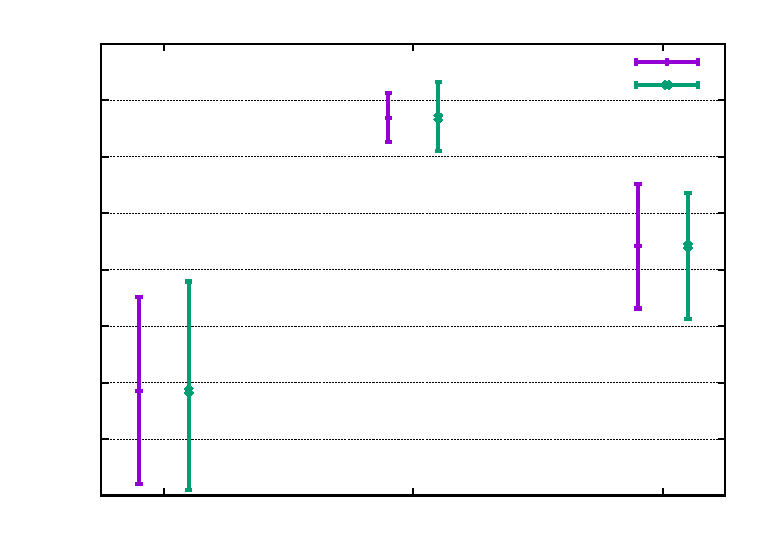
\includegraphics{AnglePlot}}%
    \gplfronttext
  \end{picture}%
\endgroup

\caption{Results of the contact angle measurements, showing average and  respectively standard deviation or range}
\label{fig:results}
\end{figure}



\subsubsection{Sources of Errors}

There are several sources of errors which could explain the wide range of measured values such as surface roughness, water evaporation and incomplete relaxation. The last two sources are convoluted and compounded by operator timing and mode of operation as explained in the following.
When the drop precipitates on the sample it must first relaxes in finite time to assume the equilibrium position, hence if the measurement is taken to early it will deviate toward a more hydrophobic angle.
On the other hand if the drop is left on the surface too long the effects of evaporation become noticeable. In this case the sides remain fixed and the ape is lowered. This gives a more hydrophilic appearance.
As the liquid drop profiles were taken from snapshots dynamic effects are negligible however the timing is crucial to the error. An early snapshot would introduce a incomplete relaxation effect, a late snapshot would induce a evaporation error. As the timing of the snapshot is manual this depends heavily on the operator hence the large variation in error.
We believe this to be the largest source of error in our measurement, as the surface roughness should not change much at different points on the sample. Measurement accuracy and uniformity could be improved by precisely controlling the timing through automatization or reducing evaporation through climate control.
